\section{Стабілізація відео}
\begin{frame}
  \frametitle{Стабілізація відео}

  Оскільки дошка~---~це плоска поверхня, ми можемо знайти матрицю гомографії між двома кадрами.
  Для цього використовуємо алгоритм SIFT та RANSAC.
  \begin{figure}[H]
    \centering
    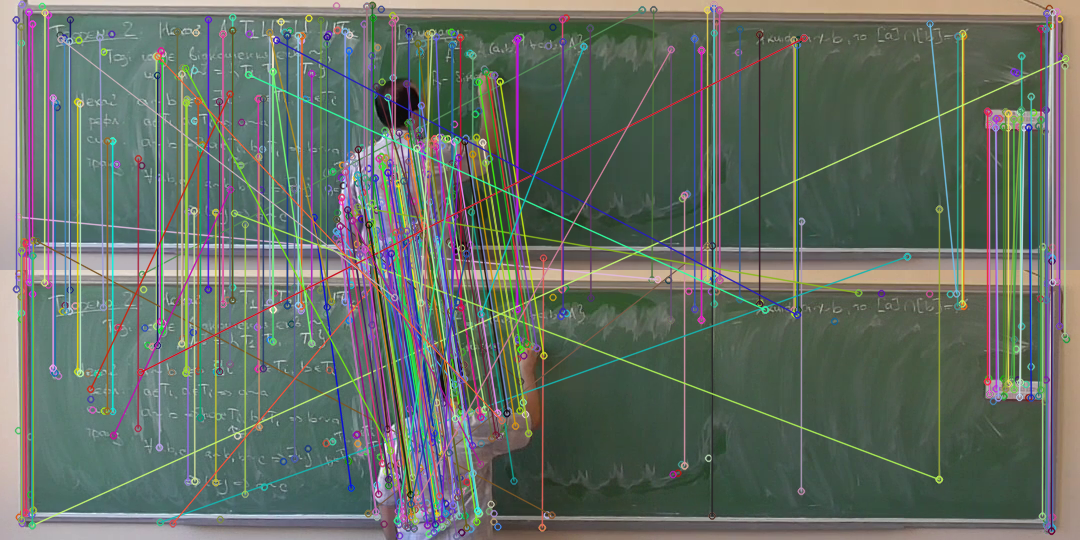
\includegraphics[width=0.55\textwidth]{images/matches_img}
    %\caption{}
  \end{figure}
  \begin{center}
    Кадри $F^i$ (верхній) та $F^{i+s}$ (нижній) із ключовими точками та лініями,\\
    які поєднують відповідні точки. \\
    Джерело ~---~ \url{https://youtu.be/a7TUp4p-pIk}
  \end{center}
\end{frame}
